\documentclass[12pt, a4paper]{article}

\usepackage{balance}
\setlength{\columnsep}{1 \baselineskip}

\newenvironment{Figure}
  {\par\medskip\noindent\minipage{\linewidth}}
  {\endminipage\par\medskip}

\usepackage{caption}

\usepackage[utf8]{inputenc}
\usepackage[english]{babel}

\usepackage[font=small,labelfont=bf]{caption}

\usepackage{amsmath}

\interdisplaylinepenalty = 2500

\usepackage{mathtools}

\usepackage{amssymb}

%\usepackage{stmaryrd}

\usepackage{amsthm}

%\usepackage{latexsym}

\usepackage{IEEEtrantools}

\usepackage{eucal}

\usepackage{bbm}

\usepackage{scalerel}

\usepackage[dvipsnames]{xcolor}
\definecolor{darkgreen}{RGB}{35, 89, 52}
\definecolor{paleorange}{RGB}{255, 236, 207}
\definecolor{paleteal}{RGB}{223, 245, 243}
\definecolor{palered}{RGB}{255, 234, 232}

\usepackage{graphicx}
\graphicspath{ {./images/} }

\usepackage{tikz}
\usetikzlibrary{arrows}
\usepackage{tikz-cd}

\usepackage{hyperref}
\hypersetup{
	colorlinks=true,
	linkcolor=darkgreen,
	filecolor=magenta,      
	urlcolor=MidnightBlue,
	citecolor=darkgreen,
	pdftitle={Dynamic codesign in Poly},
	bookmarks=true
}


\usepackage[
backend=bibtex,
maxbibnames=50,
style=alphabetic,
citestyle=alphabetic]{biblatex}
\addbibresource{candoc.bib}
%Remove In: from journal articles
\renewbibmacro{in:}{%
  \ifentrytype{article}{}{\printtext{\bibstring{in}\intitlepunct}}}


\theoremstyle{definition}

\newtheorem{counter}{Definition}[section]

\newtheorem{definitionx}[counter]{Definition}
\newenvironment{definition}
  {\pushQED{\qed}\renewcommand{\qedsymbol}{$\triangleleft$}\definitionx}
  {\popQED\enddefinitionx}

\theoremstyle{plain} 
\newtheorem{lemma}[counter]{Lemma}

\theoremstyle{plain} 
\newtheorem{proposition}[counter]{Proposition}

\theoremstyle{plain}
\newtheorem{theorem}[counter]{Theorem}

\theoremstyle{plain}
\newtheorem{question}[counter]{Question}

\theoremstyle{plain}
\newtheorem{problem}[counter]{Problem}

\theoremstyle{remark}

\newtheorem{examplex}[counter]{Example}
\newenvironment{example}
  {\pushQED{\qed}\renewcommand{\qedsymbol}{$\diamond$}\examplex}
  {\popQED\endexamplex}

\newtheorem*{excont}{Example \continuation}
\newcommand{\continuation}{??}
\newenvironment{continueexample}[1]
{\renewcommand{\continuation}{\ref{#1}}\excont[continued]}
{\endexcont}

\theoremstyle{remark}
\newtheorem{remark}[counter]{Remark}

\usepackage[most]{tcolorbox}
\newtcbtheorem[number within=section]{tcdefinition}{Definition}{colback=paleteal,colframe=NavyBlue,fonttitle=\bfseries, breakable, enhanced}{def}

\newtcbtheorem[number within=section, use counter from = tcdefinition]{tctheorem}{Theorem}{colback=paleteal,colframe=NavyBlue,fonttitle=\bfseries, breakable, enhanced}{thm}

\newtcbtheorem[number within=section, use counter from = tcdefinition]{tcexample}{Example}{colback=paleorange,colframe=BurntOrange,fonttitle=\bfseries, breakable, enhanced}{ex}

\newtcbtheorem[]{tcproblem}{Problem}{colback=palered,colframe=Bittersweet,fonttitle=\bfseries, breakable, enhanced}{pr}

\newcommand{\zuz}[1]{%
	
	\begin{tikzpicture}[#1]%
	
	\draw[semithick, line cap = round, line join = round] (-0.3ex,0.35ex) -- (0.5ex,0.35ex);
	
	\draw[semithick, line cap = round, line join = round] (0.5ex,0.35ex) -- (0.5ex,-0.5ex);
	
	\draw[semithick, line cap = round, line join = round] (0.5ex,-0.5ex) -- (1.5ex,-0.5ex);
	
	\draw[semithick, line cap = round, line join = round] (0,0) -- (1ex,0);%
	
	\draw[semithick, line cap = round, line join = round] (1ex,0) -- (1ex,-0.85ex);
	
	\draw[semithick, line cap = round, line join = round] (1ex,-0.85ex) -- (1.8ex,-0.85ex);
	
	\end{tikzpicture}%
	
} 

\renewcommand\qedsymbol{\zuz{scale=1.5}}

\newcommand{\mc}[1]{\mathcal{#1}}

\newcommand{\sub}{\subseteq}

\newcommand{\upper}{\mathsf{U}}
\newcommand{\upc}[1]{\uparrow{#1}}

\newcommand{\low}{\mathsf{L}}
\newcommand{\lwc}[1]{\downarrow{#1}}

\newcommand{\op}[1]{#1^{\text{op}}}

\newcommand{\slens}[2]{\raisebox{0.4ex}{\scaleobj{0.25}{\begin{pmatrix} \scaleobj{3}{{#1}} \\ \scaleobj{3}{{#2}} \end{pmatrix}}}}
\newcommand{\lens}[2]{\scaleobj{0.6}{\begin{pmatrix} \scaleobj{1.3}{{#1}} \\ \scaleobj{1.3}{{#2}} \end{pmatrix}}}
\newcommand{\blens}[2]{\scaleobj{0.9}{\begin{pmatrix} {#1} \\ {#2} \end{pmatrix}}}

\makeatletter
\def\slashedarrowfill@#1#2#3#4#5{%
	$\m@th\thickmuskip0mu\medmuskip\thickmuskip\thinmuskip\thickmuskip
	\relax#5#1\mkern-7mu%
	\cleaders\hbox{$#5\mkern-2mu#2\mkern-2mu$}\hfill
	\mathclap{#3}\mathclap{#2}%
	\cleaders\hbox{$#5\mkern-2mu#2\mkern-2mu$}\hfill
	\mkern-7mu#4$%
}
\def\rightslashedarrowfill@{%
	\slashedarrowfill@\relbar\relbar\mapstochar\rightarrow}
\newcommand\xslashedrightarrow[2][]{%
	\ext@arrow 0055{\rightslashedarrowfill@}{#1}{#2}}
\makeatother

\newcommand{\prof}{\xslashedrightarrow{}}

\title{Dynamic codesign in \textsf{Poly}}
\author{Marius Furter}


\begin{document}

\maketitle
\tableofcontents

\section{Recap of \textsf{Poly}}
Recall that a \emph{representable functor} has the form $\mathcal{C}(A,-) : \mathcal{C} \rightarrow \mathsf{Set} $. When $\mathcal{C} = \mathsf{Set}$, we will denote $\mathsf{Set}(A,-) =: y^A$ and call this a \emph{monomial}. A \emph{polynomial functor} is any functor that is isomorphic to a sum of monomials
$$p \cong \sum_{i \in I} y^{p[i]},$$
where the $(p[i])_{i \in I}$ is a family of sets, and the sum is taken to be the coproduct in the functor category $[\mathsf{Set},\mathsf{Set}]$ given by taking the component-wise disjoint union of the sets in question. Observe that if we evaluate $p$ at the singleton set $1$, we recover the indexing set of the sum
$$p(1) \cong \sum_{i \in I} 1^{p[i]} \cong \sum_{i \in I} 1 \cong I.$$
Hence we will often write $p \cong \sum_{i \in p(1)} y^{p[i]}$ to avoid always having to name the index set. The elements of $p(1)$ are called the \emph{positions} of $p$, while the elements of $p[i]$ are called the \emph{directions} at position $i$.

Since polynomial functors are functors, morphisms between them are given by natural transformations. By using the universal property of coproducts in $[\mathsf{Set},\mathsf{Set}]$ along with the Yoneda lemma, one can observe that
\begin{IEEEeqnarray*}{rCl}
	\mathsf{Poly}(p,q) &=& \mathsf{Poly}(\sum_{i \in p(1)} y^{p[i]},\sum_{j \in q(1)} y^{q[j]}) \\
	&\cong& \prod_{i \in p(1)} \mathsf{Poly}(y^{p[i]},\sum_{j \in q(1)} y^{q[j]}) \\
	&\cong& \prod_{i \in p(1)} \sum_{j \in q(1)} {p[i]}^{q[j]}
\end{IEEEeqnarray*}
The latter expression can be interpreted in terms of dependent products and sums: For every $i \in p(1)$ there exists $j \in q(1)$ with associated function $q[j] \rightarrow p[i]$. In other words, a morphism in $\mathsf{Poly}$ may be identified with a function $f: p(1) \rightarrow q(1)$ on positions, along with a family of functions $(f_i)_{i \in p(1)}$ where $f_i: q[f(i)] \rightarrow p[i]$ is a function on directions. This family can be expressed more concisely by assembling it into a dependent function $f^\sharp: (i \in I) \rightarrow q[f(i)] \rightarrow p[i]$.

\subsection{Lenses in $\mathsf{Poly}$}
We can express lenses in $\mathsf{Set}$ within $\mathsf{Poly}$ as maps between special types of polynomials. Let us generalize the term \emph{monomial} to include polynomials of the form $\sum_{i \in S} y^{A} \cong S y^A$, where the direction sets are independent of the positions. Now consider a morphism
$$\lens{f^\sharp}{f} :A^+ y^{A^-} \rightarrow B^+ y^{B^-} .$$
This consists of an on-positions function $f: A^+ \rightarrow B^+$ and an on-directions dependent function $f^\sharp : (a^+ \in A^+) \rightarrow B^- \rightarrow A^-$. However, since the direction sets are independent of the positions, this is just a regular function and can be curried to $f^\sharp: A^+ \times B^- \rightarrow A^-$. We now recognize that this is just a lens
$$\lens{f^\sharp}{f} : \lens{A^-}{A^+} \leftrightarrows \lens{B^-}{B^+}.$$

\subsection{Operations in $\mathsf{Poly}$}
$\mathsf{Poly}$ has four monoidal operations $+, \times,\circ,$ and $\otimes$, where $\times$ and $\otimes$ are monoidal closed. The first two are simply the categorical coproduct and product, respectively. For $p = \sum_{i \in p(1)} y^{p[i]}$ and $q = \sum_{j \in q(1)} y^{q[j]}$ these are given by the familiar addition and multiplication of polynomials:
$$p + q = \sum_{i \in p(1)} y^{p[i]} + \sum_{j \in q(1)} y^{q[j]},$$
$$p \times q = \sum_{i \in p(1)}\sum_{j \in q(1)} y^{p[i]+q[j]}.$$

On the other hand, $\circ$ is just functor composition, which corresponds to variable substitution for polynomials. It can be computed as
$$p \circ q \cong \sum_{i \in p(1)} \prod_{d \in p[i]} \sum_{j \in q(1)} \prod_{e \in q[j]} y .$$

Finally, $\otimes$ is given by multiplying both the postitions and directions:
$$p \otimes q = \sum_{i \in p(1)} \sum_{j \in q(1)} y^{p[i]q[j]}.$$
In fact, if we tensor two lenses 
$$\lens{f^\sharp}{f} :A^+_1 y^{A^-_1} \rightarrow B^+_1 y^{B^-_1} .$$
$$\lens{g^\sharp}{g} :A^+_2 y^{A^-_2} \rightarrow B^+_2 y^{B^-_2} .$$
we get a lens
$$(A^+_1 \times A^+_2)  y^{A^-_1 \times A^-_2} \rightarrow (B^+_1 \times B^+_2)y^{B^-_1 \times B^-_2}$$
which recovers the usual tensor product of lenses.

\subsection{Mode-dependence}
We have seen that we can model lenses as polynomial morphisms 
$$\lens{f^\sharp}{f} :A^+ y^{A^-} \rightarrow B^+ y^{B^-} .$$
Translating a lens representing a dynamical system thus yields a morphism
$S y^S \rightarrow O y^I$. We obtain mode-dependent systems by generalizing the former to morphisms of the type $S y^S \rightarrow q$, where $q$ is an arbitrary polynomial. Let us see how this differs from what we had before.

To specify a map $\sum_{s \in S} y^S \cong S y^S \rightarrow \sum_{j \in q(1)} y^{q[j]}$ we must give a function $f: S \rightarrow q(1)$ on positions and a dependent function $f^\sharp: (s \in S) \rightarrow q[f(s)] \rightarrow S$ on directions. We still think of the elements of $q(1)$ as outputs. The passback function $f^\sharp$ now additionally takes into account what the current output is, since it goes from $q[f(s)] \rightarrow S$ for each $s \in S$. In other words, the possible inputs a system can receive now depend on what the current output is.

\section{Codesign in \textsf{Poly} via lower sets}

\subsection{Preliminaries}
Let $P$ be a preorder whose objects we interpret as resources and whose relation $a \leq b$ means that being able to provide $b$ implies being able to provide $a$. A feasibility relation $\Phi: F \prof R$ is then a monotone function $\op{F} \times R \rightarrow \mathsf{Bool}$. Observe that
\begin{IEEEeqnarray*}{rCl}
    \hom(\op F \times R, \mathsf{Bool}) & \cong & \hom(R, \hom(\op F, \mathsf{Bool})) \\
    & \cong & \hom(R, \low F)
\end{IEEEeqnarray*}
Consider a monotone map $\varphi: \low R \rightarrow \low F$ which preserves unions. This induces a monotone map $\bar \varphi: R \rightarrow \low F$ by $\bar \varphi(r) := \varphi(\lwc r)$, where $\lwc r$ denotes the lower closure of $\{r\}$. On the other hand, if we have a monotone map $\psi: R \rightarrow \low F$ we can extend it in a unique way to a monotone map $\tilde \psi: \low R \rightarrow \low F$ which preserves unions by setting $\tilde \psi (\lwc s) := \psi(s)$ on principal lower sets. Then $\tilde \psi(S) = \tilde \psi(\bigcup_{s \in S} \lwc s) = \bigcup_{s \in S} \tilde \psi(\lwc s) = \bigcup_{s \in S} \psi(s)$. Since these operations are inverse to one another we have shown that 
$$ \hom(R, \low F) \cong \{\varphi \colon \low R \rightarrow \low F : \varphi \text{ monotone and preserves unions.}\} $$
Combining with the above, this shows that feasibility relation are just union preserving monotone functions $\low R \rightarrow \low F$. Moreover, the composition of such functions is again monotone and preserves unions. This justifies restricting out attention to monotone maps with this special property.

(Late night ramblings, Check this!)(Ordering the lower sets by inclusion makes the union a join. Hence we are considering join-preserving monotone maps in the category of distributive lattices. We can think of the above correspondence as being a functor (show this!) from \textsf{DP} to the category of distributive lattices with join-preserving maps. The fact that there is a bijection between feasibility relations and join-preserving monotone maps shows that it is faithful. By Birkhoff's representation theorem, any finite distributive lattice is isomorphic to the lower sets of some partial order (and hence preorder). Therefore, the functor is also essentially surjective if we restrict our attention to finite design problems and finite distributive lattices.)

\subsection{Basic Setup}
Let $f_t: A_t \rightarrow B_t$ be a family of functions between sets indexed by $t \in T$. Moreover, let $u_t: A_t \rightarrow T$ be a family of function indexed by $T$. We interpret $T$ as a (branching) timeline. If at time $t \in T$ we choose to transform $a \in A_t$ to $f_t(a) \in B_t$, then the timeline advances to $u_t(a) \in T$. 

We can view this data as a directed graph with vertices $(f_t, t)$ for $t \in T$ where any vertex $(f_t,t)$ has edges emanating from it indexed by $A_t$. The vertices of this graph are interpreted as the transformations $f_t: A_t \rightarrow B_t$ that are available to us at time $t$. Using $f_t$ on $a \in A_t$ advances time to $u_t(a)$ where we now have $f_{u_t(a)}: A_{u_t(a)} \rightarrow B_{u_t(a)}$ available to us.

\begin{tcexample}{Linear time}{lin-time}
    To model linear time we set $T := \mathbb{N}$ and put $u_t : A_t \rightarrow T$ to be $u_t(a) = t+1$ for all $a \in A_t$ and $t \in T$. The resulting graph looks like this:


\end{tcexample}

\begin{tcexample}{Branching time}{branch-time}
    Our model for time can accommodate branching which depends on our choices. Let $T := \{(n,i) : n \in \mathbb{N}, 1 \leq i \leq 2^n \}$, and let $A_t := \{0,1\}$ for all $t \in T$. We can now consider the branching tree:

\end{tcexample}

We now encode this data in a mode-dependent system in \textsf{Poly} with states
$$ S := \{ (f_{u_t(a)}, f_t(a)) : a \in A_t \}.$$
The input set at time $t$ will be $A_t$ and the output set $B_t$. This means that we are considering the system
$$ S y^S \rightarrow \sum_{t \in T} B_t y^{A_t}$$
with on-positions map $(f_{u_t(a)}, f_t(a)) \mapsto f_t(a) \in B_t$ and on directions map $(f_t, x) \mapsto a \mapsto (f_{u_t(a)}, f_t(a))$.

We consider some special cases to illustrate this definition.
\begin{tcexample}{Time-invariant system}{time-inv-sys}
    If $T := \{* \}$, our system consist of a single function $f : A \rightarrow B$ and $u_*: A \times T \rightarrow T$ is uniquely defined. Hence our states are simply $$ S := \{ (f, f(a)) : a \in A\}.$$
    Inputting $a_1 \in A$ into the system outputs $f(a_1)$ and updates the state to $f, f(a_1))$. Now inputting $a_2 \in A$ outputs $f(a_2)$ and updates the state to $f, f(a_2))$. So our system simply behaves like the function $f$ and transforms a stream of inputs $(a_1, a_2, a_3, \ldots) \in A^{\mathbb{N}}$ into the stream $(f(a_1), f(a_2), f(a_3), \ldots)\in B^{\mathbb{N}}$.
\end{tcexample}

\begin{tcexample}{Linear time system with constant interface}{lin-time-sys}
    Now consider $T := \mathbb{N}$ with $A_t = A$, $B_t = B$ for all $t$ and set $u_t(a) = t+1$ for all $a \in A$. However let $f_t: A \rightarrow B$ be potentially different functions. Hence our states are simply $$ S := \{ (f_{t+1}, f_t(a)) : t \in \mathbb{N}, a \in A\}.$$
    Our systems always accepts inputs from $A$ and outputs into $B$. Suppose we start in the state $(f_0,x)$, where $x \in B$ is some default initial output. Then inputting $a_0 \in A$ into the systems will update the state to $(f_1,f_0(a_1))$ and cause it to output $f_0(a_0)$. Inputting $a_1 \in A$ will update the state to $(f_2,f_1(a_1))$ and output $f_1(a_1)$. So our system transforms inputs $(a_0, a_1, a_2, \ldots) \in A^{\mathbb{N}}$ into the stream $(f_0(a_0), f_1(a_1), f_2(a_2), \ldots)\in B^{\mathbb{N}}$.
\end{tcexample}

\begin{tcexample}{Linear time system with variable interfaces}{lin-var-time-sys}
    We can change what input type the linear time system above accepts by letting the input and output sets $A_t, B_t$ vary over time. Such a system transforms inputs $(a_0, a_1, a_2, \ldots) \in \prod_{t \in \mathbb{N}} A_t$ into the stream $(f_0(a_0), f_1(a_1), f_2(a_2), \ldots)\in \prod_{t \in \mathbb{N}} B_t$.
\end{tcexample}

\begin{tcexample}{Branching time system with constant interfaces}{branch-time-sys}
    Let $A_t = \{0,1\}$ and $B_t = B$ for all $t \in T := \{(n,i) : n \in \mathbb{N}, 1 \leq i \leq 2^n \}$. Our available transformations and their transitions are given by the branching graph:

    This graph is simultaneously the transition diagram for our system, where the second element in the tuple is what the system is currently outputting. Given a vertex $s$ representing a state, the available inputs correspond to the labeled edges emanating from $s$. If we input $a$ to the system, following the edge with label $a$ leads to the new state, along with its output.
\end{tcexample}

\subsection{Application to codesign}
To apply the above top codesign, we simply specialize the functions $f_i: A_i \rightarrow B_i$ to be monotone maps $\phi_i: \low R_i \rightarrow \low F_i$ which preserve unions. A nice feature is that each $\low P$ contains the emptyset which can act as a default value for input and output. Inputting the emptyset corresponds to waiting.

\begin{tcexample}{Waiting}{waiting}
    So far, each transition takes exactly one time-step which is modeled as an application of the function $u_t$. What if we want certain transformations to take longer? One way to achieve this is to close the input channel for several time-steps and only then outputting the functionality. This is illustrated by the following transition diagram:

\end{tcexample}

The problem with the above framework is that it is not possible to express the situation where a given resource $r$ can be converted either $f$ or $g$ if $f,g$ are not part of the same time-set $F_i$. This led me to rethink the above approach and come up with a better description.

\section{Codesign in \textsf{Poly} via parameterized systems}
The basic idea is that an feasibility relation must be realized by some machine which predictably converts input into output. Such a machine may have various settings that allow it to convert a given resource into several different products. If we assume that we can change the settings of the machine at will (or the service provider takes care of this), we can abstract over the settings and simply state that a resource can be converted to several products according to our choosing. After this abstraction, it looks like our machine is non-deterministic (relational), when in fact we are simply aggregating its various deterministic modes of operation.

Concretely, we will decompose a feasibility relation into a union of functions. Each of these functions will be implemented as one setting of a parameterized machine. We can then sum over the parameters to recover the feasibility relation. In this way, classic codesign will turn out to be steady-state analysis of certain time-invariant systems.

\subsection{Codesign as steady-state analysis of time-invariant systems}
Let $\Phi: R \prof F$ be a feasibility relation. Write $\Phi = \bigcup_{i \in I} \varphi_i$, where $\varphi_i: R_i \rightarrow F$ are monotone maps. In general there are many ways of doing this. It will turn out to be immaterial what decomposition is chosen, but having a smaller index set $I$ is preferable. The minimal size of $I$ is determined by $\max_{r \in R}{| \{f : \Phi(r,f) \} |}$.

We will now use the $\varphi_i$ to construct a parametrized mode-dependent system which takes inputs $(i, r) \in I \times R_i$ and outputs $\varphi_i(r)$. Formally we set $S := \{ (i,\varphi_j(r)) : i,j \in I, r \in R_j \}$, define the on-positions map to be the identity $(i,\varphi_j(r)) \mapsto (i,\varphi_j(r))$, and let the on-directions map be $(i,\varphi_j(x))\mapsto (k,r \in R_i) \mapsto (k,\varphi_i(r))$. 

In words, the system's states are transformed resources along with the current parameter setting. The systems simply outputs its state. On update, if the system is in setting $i$, it takes a resource $r \in R_i$ (mode-dependence allows us to impose this constraint) and a new parameter setting $j$. It then transforms the resource into $\varphi_i(r)$ using the map corresponding to its setting and then updates its setting $i \rightsquigarrow j$.

\begin{tcexample}{Apples and Oranges}{apple-orange}

\end{tcexample}

\subsubsection{Steady-state matrices}
We will now look at the steady-states of our system. For this we first need to define charts and behaviors for our mode-dependent systems.

\begin{tcdefinition}{Chart}{chart}
	Let $\lens{A^-_{a \in A^+}}{A^+}$ and $\lens{B^-_{b \in B^+}}{B^+}$ be dependent sets. Then a chart $\lens{f_\flat}{f} \colon \lens{A^-_{a \in A^+}}{A^+} \rightrightarrows \lens{B^-_{b \in B^+}}{B^+}$ consists an on-position function $f \colon A^+ \rightarrow B^+$ and an a family of on-direction functions $f_{\flat,a} \colon A^-_a \rightarrow B^-_{f(a)}$.
\end{tcdefinition}

\begin{tcdefinition}{Behavior}{behavior}
	Let $\mc{S}$ and $\mc{T}$ be mode-dependent systems and $$\lens{f_\flat}{f} \colon \lens{I^S_{o \in O^S}}{O^S} \rightrightarrows \lens{I^T_{o \in O^T}}{O^T}$$
	a chart between their interfaces. An \emph{$\lens{f_\flat}{f}$-behavior of shape $\mc{S}$ in $\mc{T}$} is a map $\phi: S \rightarrow T$ such that for all $s \in S$ and $i \in I^S_{out_S(s)}$
	$$out_T(\phi(s)) = f(out_S(s)), $$
	$$\phi(up_S(s,i)) = up_T(\phi(s), f_{\flat,out_S(s)}(i)).$$
\end{tcdefinition}

\begin{tcdefinition}{Steady-state}{steady-state}
	Let $\mc{S} := \lens{up_S}{out_S} \colon \lens{S_{s \in S}}{S} \leftrightarrows \lens{I_{o \in O}}{O}$ and consider the system $\mc{B} \colon \lens{*}{*} \leftrightarrows \lens{*}{*}$ whose maps are all trivial. A chart $\lens{f_\flat}{f} \colon \lens{*}{*} \rightrightarrows \lens{I_{o \in O}}{O}$ consists of functions $f \colon * \rightarrow O$ and $f_{\flat,*} \colon * \rightarrow I_{f(*)}$. In other words, we a simply selecting $o \in O$ and $i \in I_o$. 

	An $i,o$-steady-state now consists of an $\lens{i}{o}$-behavior of shape $\mc{B}$ in $\mc{S}$. This is a function $\phi \colon * \rightarrow S$, which we will identify with $\phi(*) = s \in S$, such that for all $x \in *$ and $i \in *$ we have
	$$out(s) = o, $$
	$$s = up(s,i).$$
\end{tcdefinition}

For $\mc{S} \colon \lens{S_{s \in S}}{S} \leftrightarrows \lens{I_{o \in O}}{O}$ we can gather together all steady-states in a dependent function $M: O \rightarrow I_{o \in O} \rightarrow \mathsf{P}S$ which assigns each $i,o$-pair the set of $i,o$-steady-states. We can think of $M$ as a matrix which has entries $m_{i,o}$ for $o \in O$ and $i \in I_o$.

It turns out that steady-state matrices compose according to matrix arithmetic. In particular, if we put two systems in parallel we have $M_{S \otimes T} = M_S \otimes M_T $ where $(A \otimes B)_{(i,i'),(o,o')} = A_{i,o} \times B_{i',o'}$ is the Kronecker product. Moreover, if we feed the output of $S$ into $T$, the resulting system $S \triangleleft T$ has steady states $M_{S \triangleleft T} = M_S \cdot M_T$ where $(A \cdot B)_{i,j} := \sum_{k} A_{i,k} \times B_{k,j}$ is matrix multiplication.

The following partial trace operation will be of highest importance: Consider a system $\mc{S} \colon \lens{S_{s \in S}}{S} \leftrightarrows \lens{X \times I_{o \in O} }{X \times O}$ where the set $X$ serves as input under any current output. We can then wire the $X$-output of the system back into its $X$-input to obtain the system $\mc{S}^\dagger$, illustrated below:
\begin{center}
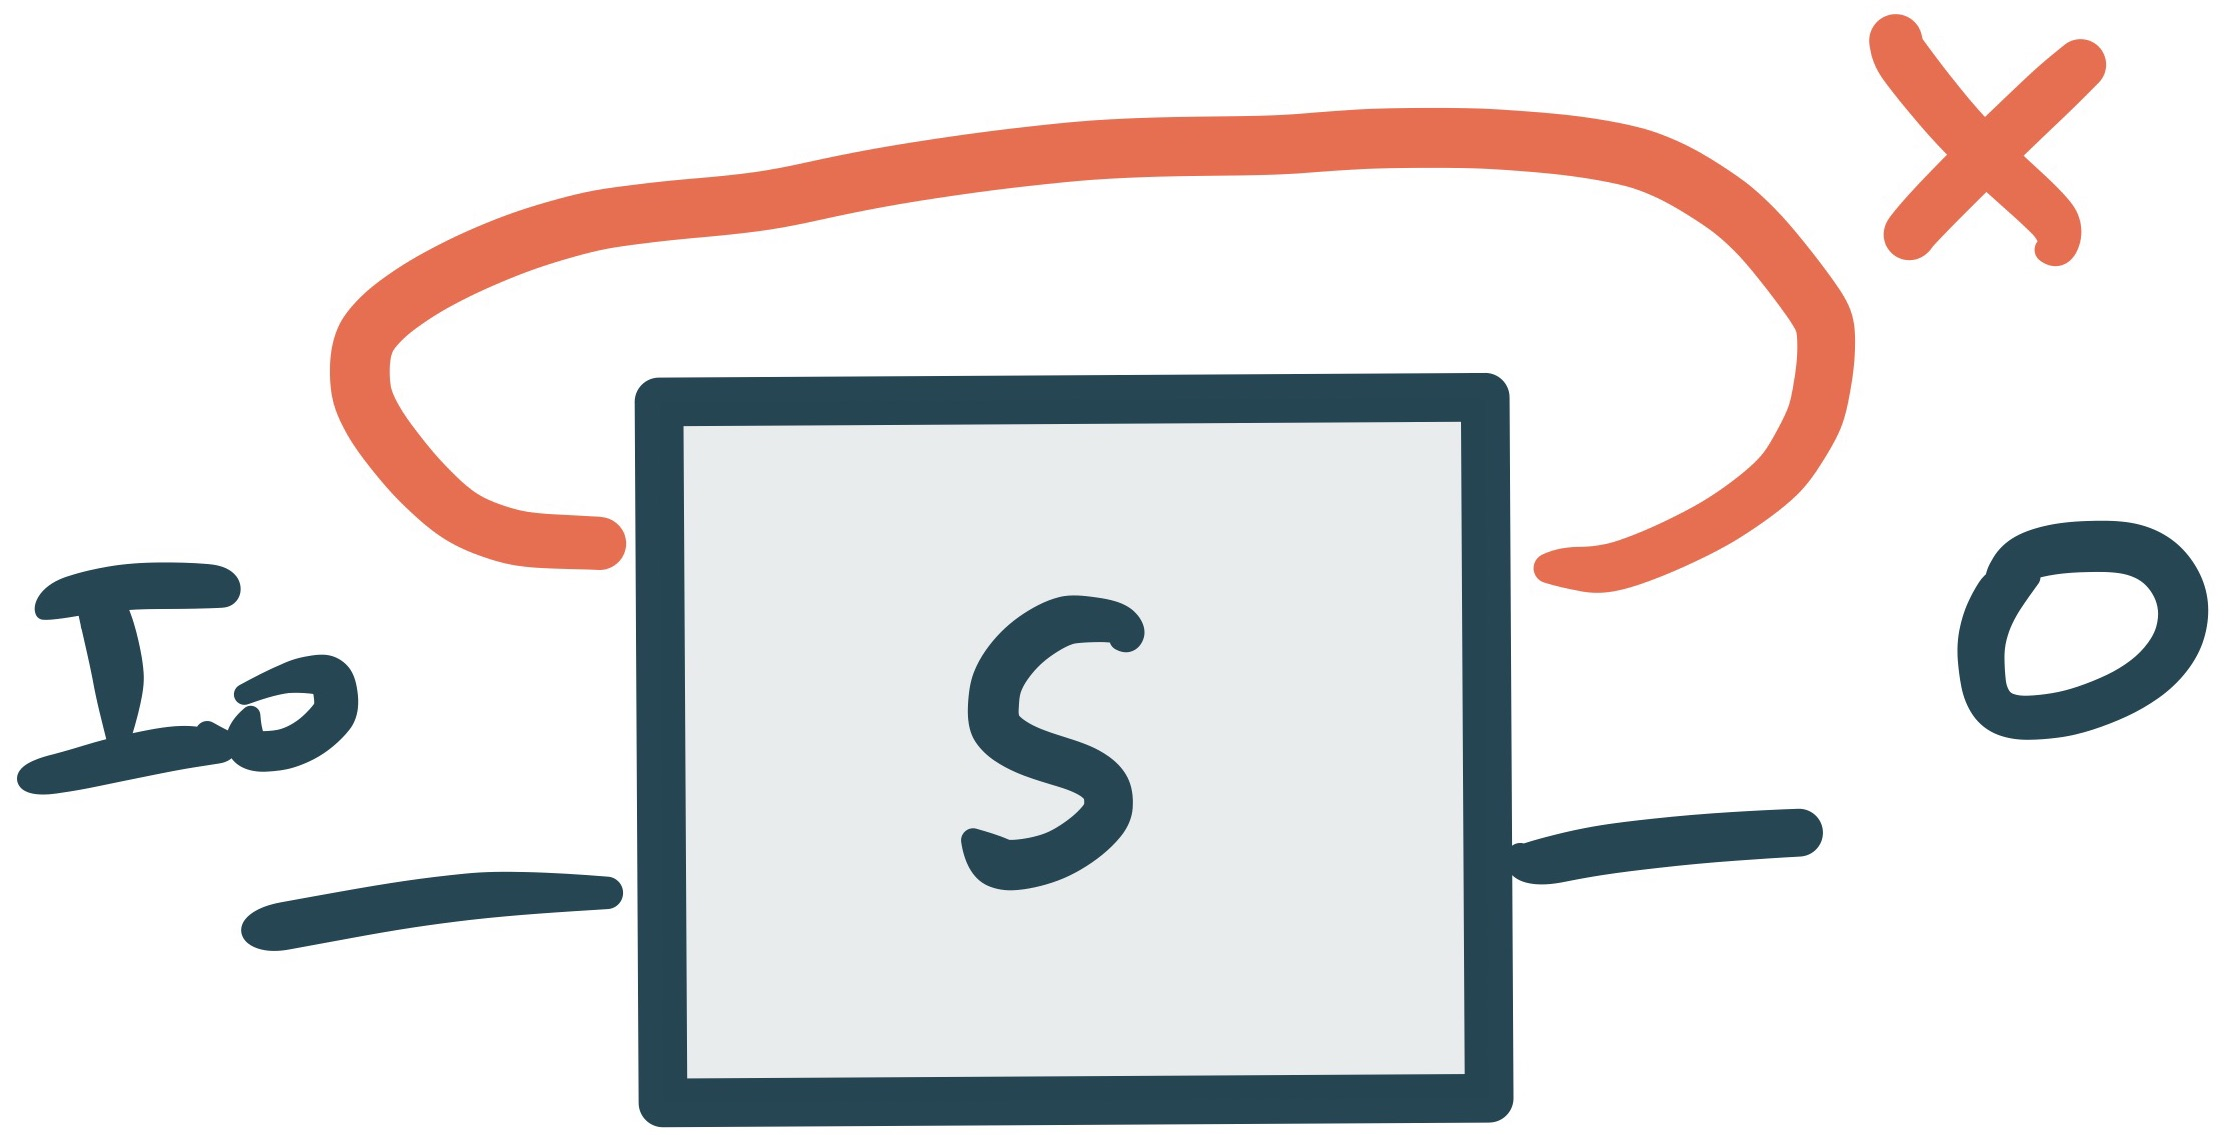
\includegraphics[width = 0.4\textwidth]{trace.jpg}
\end{center}
The update and output functions are now modified to $up_\dagger(s) = up(s,\pi_1(out(s)),i)$ and $out_\dagger(s) = \pi_2(out(s))$.

Let's think about what happens to the steady-states of $\mc{S}$ under this operation. We claim that $M_{\mc{S}^\dagger}(i,o) = \sum_{x \in X} M_{\mc{S}}(x,i)(x,o)$. To see this, consider and $i,o$-steady-state $s$ of $\mc{S}^\dagger$. This satisfies $out_\dagger(s) = o$ and $up_\dagger(s,i) = s$. By definition $out_\dagger(s) = \pi_2(out(s))$, so $out(s) = (x,o)$ for some $x$. Moreover, $s = up_\dagger(s,i) = up(s,(\pi_1(out_s),i)) = up(s,(x,i))$, so $s$ is also an $(x,i),(x,o)$-steady-state of $\mc{S}$. Conversely, any $(x,i),(x,o)$-steady-state $s$ satisfies $out(s) = (x,o)$ and $up(s,(x,i)) = s$. Hence $out_\dagger(s) = o$ and $up_\dagger(s,i) = up(s,(\pi_1(out(s)),i)) = up(s,(x,i)) = s$. So $s$ is an $i,o$-steady-state of $\mc{S}^\dagger$. 

\subsubsection{Back to codesign}
We can now apply the above ideas to the parametrized system $\mc{P}$ representing to feasibility relation $\Phi: R \prof F$. Recall that we wrote $\Phi = \bigcup_{i \in I} \varphi_i$ as a union of monotone functions $\varphi_i \colon R_i \rightarrow F$. Then the system takes inputs $(i, r) \in I \times R_i$ and outputs $\varphi_i(r)$. It has states $S := \{ (i,\varphi_j(r)) : i,j \in I, r \in R_j \}$, with identity on-positions map $(i,\varphi_j(r)) \mapsto (i,\varphi_j(r))$, and on-directions map $(i,\varphi_j(x))\mapsto (k,r \in R_i) \mapsto (k,\varphi_i(r))$.

Observe that an $(i,r),(j,f)$-steady-state of $\mc{P}$ is $s = (i,\varphi_j(r))$ satisfying $(j,f) = out(s) = (i,\varphi_j(r))$ and $s = up(s,(i,r)) = (i,\varphi_i(r))$. Hence $j=i$ and $f = \varphi_i(r)$. Therefore
$$M_\mc{P}(i,r)(j,f) = \begin{cases} (i,\varphi_i(r)), & \text{if } i=j \text{ and } \varphi_i(r) = f, \\ \emptyset, & \text{else.} \end{cases} $$

We now plug the output parameter $i \in I$ back as input into the system to get $\mc{P}^\dagger$:
\begin{center}
	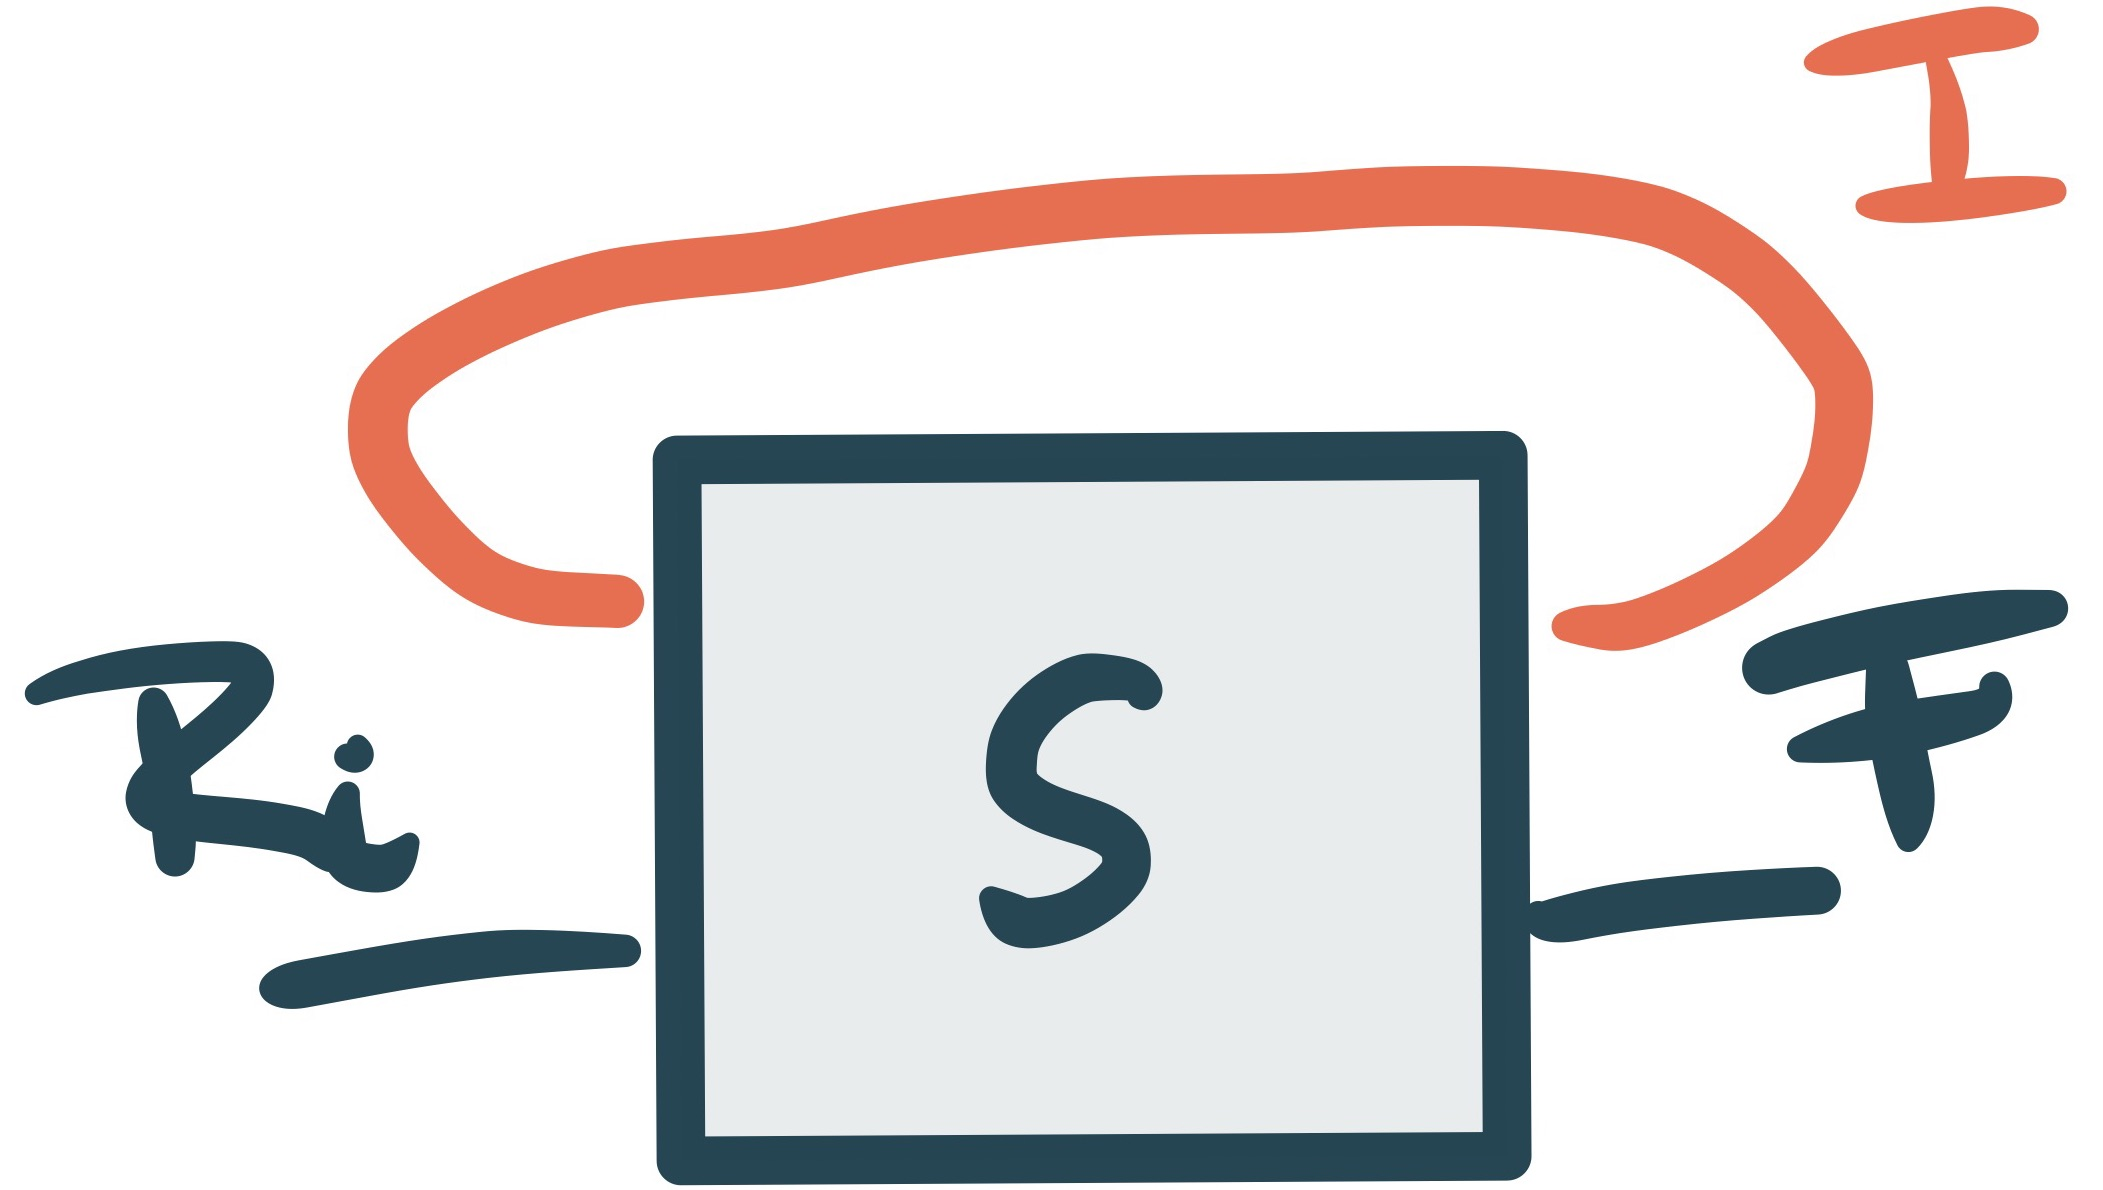
\includegraphics[width = 0.4\textwidth]{parameter-trace.jpg}
\end{center}

The steady states of $\mc{P}^\dagger$ are given by
\begin{IEEEeqnarray*}{rCl}
	M_{\mc{P}^\dagger}(r,f) &=& \sum_{i \in I} M_\mc{P}(i,r)(i,f) \\
	&=& \sum_{i \in I} \begin{cases} (i,\varphi_i(r)), & \text{if } i=j \text{ and } \varphi_i(r) = f, \\ \emptyset, & \text{else.} \end{cases} \\
	&=& \sum_{i \in I} \{(i,\varphi_i(r)) : \varphi_i(r) = f\}.
\end{IEEEeqnarray*}
Hence $M_{\mc{P}^\dagger}(r,f)$ is non-empty iff $\varphi_i(r) = f$ for some $i$ iff $\Phi(r,f)$ is feasible. So $M_{\mc{P}^\dagger}$ is essentially just the matrix associated to the relation $\Phi$ (although the matrix could contain sets with multiple elements if our decomposition of $\Phi$ was not disjoint). We will interpret $M_{\mc{P}^\dagger}(r,f)$ as the set of ways to transform $r$ into $f$. Hence we have shown that we can encode a feasibility relation $\Phi$ into a system $\mc{P}$ whose steady states are precisely the transformations of $\Phi$.

Now let $\mc{P}$ be a system representing $\Phi: R \prof F$ and $\mc{Q}$ be a system representing $\Psi: F \prof G$. The matrix of steady-states of the sequential composite can be calculated by $M_{\mc{P} \triangleleft \mc{Q}} = M_{\mc{P}} \cdot M_\mc{Q}$ where $M_{\mc{P}} \cdot M_\mc{Q}(r,g) = \sum_{f \in F} M_{\mc{P}}(r,f) \times M_\mc{Q}(r,g)$. On the other hand, $\Psi \circ \Phi (r,g) = \bigvee_{f \in F} \Phi(r,f) \wedge \Psi(f,g)$. So the sequential composite $\mc{P} \triangleleft \mc{Q}$ has almost the same steady-states as a system representing $\Psi \circ \Phi$. The only difference is that the sequential composition of systems also keeps track of the possible ways on can transform $r$ into $g$.

We also have compatibility with the parallel product: If $\mc{P}$ represents $\Phi: R \prof F$ and $\mc{Q}$ represents $\Psi: R' \prof F'$, then the steady-states of the parallel product $\mc{P} \otimes \mc{Q}$ are given by $M_{P \otimes Q}((r,r'),(f,f')) = M_P(r,f) \times M_Q(r',f')$. On the other hand, $\Phi \otimes \Psi ((r,r'),(f,f')) = \Phi(r,f) \wedge \Psi(r',f')$. This shows that the $M_{P \otimes Q}$ is the same as the steady-state matrix of a system representing $\Phi \otimes \Psi$.

\begin{question}
	What system has the disjoint union of the steady states of its components? This would amount to taking the direct sum of the steady-state matrices.
\end{question}

Answer: Let $\mc{S} := \lens{up_S}{out_S} \colon \lens{S_{s \in S}}{S} \leftrightarrows \lens{I_{o \in O}}{O}$ and $\mc{T} := \lens{up_T}{out_T} \colon \lens{T_{t \in T}}{T} \leftrightarrows \lens{J_{u \in U}}{U}$. Define $\mc{S} \sqcup \mc{T} \colon \lens{S \sqcup T}{S \sqcup T} \leftrightarrows \lens{I_o \sqcup J_u}{O \sqcup U}$ with on-positions function 
$$x \mapsto \begin{cases} out_S(x) & x \in S \\ out_T(x) & x \in T. \end{cases}$$ 
and on-directions function 
$$ x \mapsto \begin{cases} i \in I_x \mapsto up_S(x,i) & x \in S \\ j \in J_x \mapsto up_T(x,j) & x \in T. \end{cases}$$
The steady-state matrix of this system will satisfy 
$$M_{S \sqcup T}(x,y) = \begin{cases} M_S(x,y) & y \in O, x \in I_o \\  M_T(x,y) & y \in U, x \in J_u \\ \emptyset & \text{else.} \end{cases} = M_S \oplus M_T.$$

\begin{question}
	Think about how linear algebra concepts translate: Hadamard product, inverses, spectral theorem, inner products, orthogonal matrices, norms, ect. How much of linear algebra translates to matrices valued in a monoid like $\mathbb{N}$?
\end{question}

\subsection{Introducing dynamics}

\begin{tcdefinition}{Trajectories}{trajectories}
	Let $\mc{S} := \lens{up_S}{out_S} \colon \lens{S_{s \in S}}{S} \leftrightarrows \lens{I_{o \in O}}{O}$ and consider the system $\mc{T} \colon \lens{\mathbb{N}_{n \in \mathbb{N}}}{\mathbb{N}} \leftrightarrows \lens{*}{\mathbb{N}}$ whose on-positions map is the identity and whose on-directions map sends $n \mapsto * \mapsto n+1$.

	A chart $\lens{f_\flat}{f} \colon \lens{*}{\mathbb{N}} \rightrightarrows \lens{I_{o \in O}}{O}$ consists of a sequence $f \colon \mathbb{N} \rightarrow O$ and a family of maps $f_{\flat,n} \colon * \rightarrow I_{f(n)}$. We can identify the latter with a sequence $(a_0, a_1, \ldots)$ where each $a_i \in I_{f(i)}$.

	Given sequences $o \in \prod_{n \in \mathbb{N}} O$ and $i \in \prod_{n \in \mathbb{N}} I_{o(n)}$, an $i,o$-trajectory in $\mc{S}$ consists of a sequence $s \colon \mathbb{N} \rightarrow S$ such that for all $n \in \mathbb{N}$ we have
	$$out(s(n)) = o(n), $$
	$$s(n+1) = up(s(n), i(n)).$$
\end{tcdefinition}

\end{document}